\documentclass[../main/report.tex]{subfiles}
\begin{document}
\chapter{System Overview}

\section{Logical System Structure}
\begin{figure}[H]
	\centering
	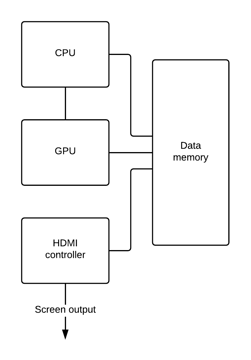
\includegraphics[width=0.5\textwidth]{../system_overview/diagrams/logical_overview.png}
	\caption{Logical overview of the system.}
	\label{fig:logical_overview}
\end{figure}


A conceptual overview of the Demolicious computer is depicted in figure \ref{fig:logical_overview}.
On a large scale, it is made up of a CPU and a GPU.
In addition, an external memory chip is used for storing framebuffers for screen output.
A dedicated HDMI module reads pixel data from the framebuffer and displays it on screen.

\section{Programming Model}
\subfile{../system_overview/programming_model}

\end{document}
